\chapter{Deep Equilibrium Models}
\label{chapter:deep_equilibrium_models}

\section{Steady State Problems}
\label{sec:steady_state_problems}

Steady State Problems involve determining the equilibrium state of a system, i.e., the state of the system where the rate of change of the system is zero. Let, our steady state problem be defined as follows:
%
\begin{equation}
  \frac{\partial z}{\partial t} = \func{f_\theta}{z, t} - z
\end{equation}
%
In case of continuous dynamical systems, the steady state would be determined by the partial derivative w.r.t. time being zero:
%
\begin{equation}
  \frac{\partial z}{\partial t} = 0
\end{equation}
%
In case of discrete dynamical systems, the steady state would be defined by states remaining constant over time:
%
\begin{equation}
  z_{n + 1} = z_n \implies \zstar = \func{f_\theta}{\zstar, \infty}
\end{equation}
%
There are two ways to solve steady state problems:
%
\begin{enumerate}
  \item \textbf{Treating it as a Nonlinear Problem}: \todo{}
  \item \textbf{Treating it as an ODE}: \todo{}
  \item \textbf{Using Pseudo-Transient Methods}: \todo{}
\end{enumerate}
%

% \todo{\url{https://docs.sciml.ai/NonlinearSolve/stable/solvers/SteadyStateSolvers/}}

\section{Sensitivity Analysis of Steady State Problems}
\label{sec:sensitivity_analysis_ssproblems}

Let, $\zstar$ be the steady state solution of the system, i.e., $\zstar = \func{f_\theta}{\zstar, \infty}$. For the sake of brevity, let us drop the $t = \infty$ term, i.e., $\zstar = \func{f_\theta}{\zstar}$. Differentiating w.r.t. $\theta$ we get:
%
\begin{align}
           & \frac{\partial \zstar}{\partial \theta} = \frac{\partial \func{f_\theta}{\zstar}}{\partial \zstar} \times \frac{\partial \zstar}{\partial \theta} + \frac{\partial \func{f_\theta}{\zstar}}{\partial \theta}\\
  \implies & \left( I - \frac{\partial \func{f_\theta}{\zstar}}{\partial \zstar} \right) \times \frac{\partial \zstar}{\partial \theta} = \frac{\partial \func{f_\theta}{\zstar}}{\partial \theta}
\end{align}
%
Let, the cost function we are optimizing be $\func{g}{\zstar, \theta}$. Taking the total derivative of $\func{g}{\zstar, \theta}$ w.r.t. the parameters $\theta$ we get:
%
\begin{align}
  \frac{d \func{g}{\zstar, \theta}}{d \theta} &= \frac{\partial \func{g}{\zstar, \theta}}{\partial \zstar} \times \frac{\partial \zstar}{\partial \theta} + \frac{\partial \func{g}{\zstar, \theta}}{\partial \theta}\\
  &= \frac{\partial \func{g}{\zstar, \theta}}{\partial \zstar} \times \left( I - \frac{\partial \func{f_\theta}{\zstar}}{\partial \zstar} \right)^{-1} \times \frac{\partial \func{f_\theta}{\zstar}}{\partial \theta} + \frac{\partial \func{g}{\zstar, \theta}}{\partial \theta} \label{eq:ss_gradient}
\end{align}
%
% Let, the size of the parameters be $L_\theta$ and the size of the states be $L_z$. The RHS of the above equation involves:
% %
% \begin{enumerate}
%   \item $\frac{\partial \func{g}{\zstar, \theta}}{\partial \theta}$: $1 \times L_\theta$ matrix
%   \item $\frac{\partial \func{g}{\zstar, \theta}}{\partial \zstar}$: $1 \times L_z$ matrix
%   \item $\left( I - \frac{\partial \func{f_\theta}{\zstar}}{\partial \zstar} \right)^{-1}$: $L_z \times L_z$ matrix
%   \item $\frac{\partial \func{f_\theta}{\zstar}}{\partial \theta}$: $L_z \times L_\theta$ matrix
% \end{enumerate}
%
% The RHS term involves the jacobian $\frac{\func{f_\theta}{\zstar}}{\partial \zstar}$ which can be computed for small systems (around $|z| < 50$) using forward mode automatic differentiation. However, as the size of the dynamical system increases (to potentially thousands of states) constructing the entire jacobian (and inverting it) is both computationally and memory-wise inefficient. Instead of directly computing the RHS, we can rewrite \Cref{eq:ss_gradient}:
The RHS term involves the inverse of the jacobian $\frac{\func{f_\theta}{\zstar}}{\partial \zstar}$, computing which is both computationally and memory-wise inefficient. Instead of directly computing the RHS, we can rewrite \Cref{eq:ss_gradient} as:
%
\begin{align}
  & \lambda^T = \frac{\partial \func{g}{\zstar, \theta}}{\partial \zstar} \times \left( I - \frac{\partial \func{f_\theta}{\zstar}}{\partial \zstar} \right)^{-1}\\
  \implies & \lambda^T \times \left( I - \frac{\partial \func{f_\theta}{\zstar}}{\partial \zstar} \right) = \frac{\partial \func{g}{\zstar, \theta}}{\partial \zstar}\\
  \implies & \left( I - \frac{\partial \func{f_\theta}{\zstar}}{\partial \zstar} \right)^T \times \lambda = \left(\frac{\partial \func{g}{\zstar, \theta}}{\partial \zstar}\right)^T \label{eq:ss_lambda_linear}
\end{align}
%
Substituting $\lambda^T$ in the \cref{eq:ss_gradient}, we get:
%
\begin{equation}
  \frac{d \func{g}{\zstar, \theta}}{d \theta} = \lambda^T \times \frac{\partial \func{f_\theta}{\zstar}}{\partial \theta} + \frac{\partial \func{g}{\zstar, \theta}}{\partial \theta} \label{eq:ss_total_gradient}
\end{equation}
%
For small systems we can compute $\frac{\partial \func{f_\theta}{\zstar}}{\partial \zstar}$ using forward mode automatic differentiation and solve \Cref{eq:ss_lambda_linear} using any linear solver. However, as the scale of the problem increases, these methods are inefficient and often practically infeasible. We defer the discussion on how to deal with large scale steady state problems to \Cref{subsec:adjoint_equations_deqs}. Hence, sensitivity analysis of a (small) steady state problem boils down to solving a linear system of equations and a matrix-vector product.


\section{Deep Equilibrium Networks}
\label{sec:deep_equilibrium_networks}

\begin{figure}[t]
  \centering
  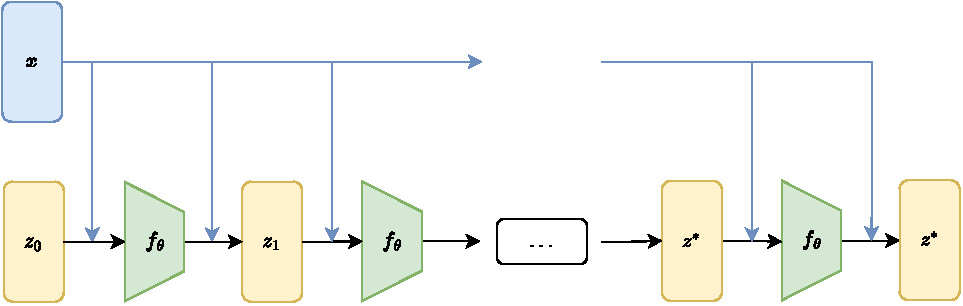
\includegraphics[width=0.9\textwidth]{../figures/deep_equilibrium_models/model_architecture.pdf}
  \caption{\textbf{Discrete DEQ Formulation}: Discrete DEQ Block where the input $x$ is injected at every iteration till the system (with initial state $z_0$) converges to a steady $\zstar$.}
  \label{fig:model_architecture_discrete_deq}
\end{figure}

Deep Equilibrium Networks (DEQs)~\citep{bai_deep_2019} are implicit models where the output space represents a steady-state solution. Intuitively, this represents infinitely deep neural networks with input injection, i.e., an infinite composition of explicit layers $z_{n + 1} = f_\theta(z_n, x)$ with $z_0 = 0$ and $n \rightarrow \infty$. In practice, it is equivalent to evaluating a dynamical system until it reaches a steady state $\zstar = f_\theta(\zstar, x)$.

% \citet{bai_deep_2019, bai_multiscale_2020} perform nonlinear fixed point iterations of the discrete dynamical system using Broyden's method~\citep{broyden1965class, bai_multiscale_2020} to reach this steady-state solution. 

Evaluating DEQs requires solving a steady-state equation involving multiple evaluations of the explicit layer slowing down the forward pass. However, driving the solution to steady-state makes the backward pass very efficient~\citep{johnson2012notes} (See \Cref{sec:sensitivity_analysis_ssproblems}). Despite a potentially infinite number of evaluations of $f_\theta$ in the forward pass, backpropagation only requires solving a linear equation.

\subsection{Nonlinear Solvers}
\label{subsec:nonlinear_solvers_deqs}

In this section, we will exclusively discuss Nonlinear Solvers for solving large steady state problems (i.e., systems with thousands of states).

\subsubsection{Broyden's Method}
\label{subsubsec:broyden_method}

\subsubsection{Anderson Acceleration}
\label{subsubsec:anderson_acceleration}

\subsection{Limited Memory Broyden's Method}
\label{subsec:limited_memory_broyden}

\subsection{Jacobian Free Newton-Krylov Methods (JNFK) for solving Linear Systems}
\label{subsec:newton_krylov_methods}

\todo{\url{https://en.wikipedia.org/wiki/Generalized_minimal_residual_method}}

\todo{\url{https://citeseerx.ist.psu.edu/doc/10.1.1.636.3743}}

\subsection{Adjoint Equations}
\label{subsec:adjoint_equations_deqs}

In \Cref{sec:sensitivity_analysis_ssproblems}, we derived the following linear system of equations:
%
\begin{equation}
  \left( I - \frac{\partial \func{f_\theta}{\zstar}}{\partial \zstar} \right)^T \times \lambda = \left(\frac{\partial \func{g}{\zstar, \theta}}{\partial \zstar}\right)^T
\end{equation}
%
For DEQs, the state space is too large to compute the entire jacobian matrix $\frac{\partial \func{f_\theta}{\zstar}}{\partial \zstar}$. Instead of computing $ A = \left( I - \frac{\partial \func{f_\theta}{\zstar}}{\partial \zstar} \right)^T $, we can use Matrix-Free Methods discussed in \Cref{subsec:newton_krylov_methods} to solve \Cref{eq:ss_lambda_linear}. To use JFNK solvers we need to be efficiently compute:
%
\begin{align}
  A \times \lambda &= \lambda - \left( \frac{\partial \func{f_\theta}{\zstar}}{\partial \zstar} \right)^T  \times \lambda\\
  &= \lambda - \left( \lambda^T \times  \frac{\partial \func{f_\theta}{\zstar}}{\partial \zstar} \right)^T
\end{align}
%
The second term is the Vector-Jacobian Product (VJP) which can be efficiently computed by any reverse-mode automatic differentiation framework (without constructing the entire Jacobian). Additionally, in \Cref{eq:ss_total_gradient} we can compute $\lambda^T \times \frac{\partial \func{f_\theta}{\zstar}}{\partial \theta}$ using the VJP trick using any reverse-mode automatic differentiation framework.

\section{Convergence Criteria}
\label{sec:ssproblem_convergence_criteria}

\todo{\url{https://docs.sciml.ai/NonlinearSolve/stable/basics/TerminationCondition/}}

\section{Common Applications of DEQs}
\label{sec:common_applications_deqs}

\section{Accelerating DEQs}
\label{sec:accelerating_deqs}

\subsubsection{Jacobian Regularization of DEQs}
\label{subsec:jacobian_regularization_deqs}

\subsubsection{Jacobian-Free Backpropagation}
\label{subsec:jacobian_free_backpropagation}

\subsubsection{Jacobian-Free Newton-Krylov Methods}

